\newpage
% ==========================================
%              CHAPTER FOUR
% ==========================================
\thispagestyle{plain}

\begin{center}
    \vspace*{0.5cm}
    {\large \textit{Chapter Four}} \\[0.4cm]
    {\Large \textbf{4 \quad METHODOLOGY --- WORD RECOGNITION}}
\end{center}
\addcontentsline{toc}{chapter}{\textbf{4 \quad METHODOLOGY --- WORD RECOGNITION}}
\vspace{1in}

\normalsize
\startchapterfloats{4}

\noindent Chapter~3 presented letter-recognition methodology. Chapter~2 Table~\ref{tab:feature-vectors} and Table~\ref{tab:four-models} introduced the hybrid word-input design: ASL words consume buffered RGB clips; ArSL words consume 225-D normalised Holistic sequences. This chapter specifies the full preprocessing equations, model architectures, and model-side inference protocols for \textbf{both} graduation word models --- Model~3 (ASL, Inception I3D) and Model~4 (ArSL, stacked BiLSTM) --- treated symmetrically as standalone Eshara pipelines (web wiring is in Chapter~5). The chapter is divided into two halves: \textbf{Part~A} (Sections~4.1--4.5) and \textbf{Part~B} (Sections~4.6--4.9), followed by a cross-language comparison and evaluation protocol (Sections~4.10--4.12). Quantitative results are reported in Chapter~6~\cite{li2020wlasl,sidig2021karsl,zhang2020mediapipe}.\par\vspace{0.4cm}

\begin{table}[H]
\centering
\caption{Chapter~4 at a glance: side-by-side comparison of both word recognition pipelines.}
\label{tab:ch4-overview}
\small
\begin{tabular}{|P{3.0cm}|P{5.4cm}|P{5.4cm}|}
\hline
\textbf{Property} & \textbf{ASL Words (Model~3)} & \textbf{ArSL Words (Model~4)} \\
\hline
Dataset & WLASL-2000 subset & KArSL-502 (SignID 71--170) \\
Classes & 100 WLASL glosses & 100 Arabic words \\
Input tensor & $(1,3,32,224,224)$ RGB & $(1,48,225)$ Holistic \\
Frames & 32 & 48 \\
Feature source & Raw RGB pixels & MediaPipe Holistic landmarks \\
Architecture & Inception I3D (3-D CNN) & Stacked BiLSTM \\
Parameters & $\sim$12.5\,M & $\sim$255\,K \\
Checkpoint & \texttt{asl\_word\_i3d.pt} & \texttt{arsl\_word\_bilstm.h5} \\
Stabilisation & 6/10 vote, $\geq$50\,\% conf, 1.2\,s & Hand-present gate, rolling deque \\
Test Top-1 & \textbf{65.89\,\%} (WLASL-100 benchmark) & 99.62\,\% \\
\hline
\end{tabular}
\end{table}
\vspace{0.6cm}

% ==========================================================
% PART A: ASL WORD RECOGNITION
% ==========================================================
\begin{center}
\large\textbf{PART A: ASL WORD RECOGNITION (Model~3 --- Inception I3D)}
\end{center}
\addcontentsline{toc}{section}{\textbf{PART A: ASL WORD RECOGNITION (Model 3)}}
\vspace{0.4cm}
\noindent\rule{\textwidth}{0.8pt}
\vspace{0.4cm}

% --- 4.1 WLASL DATASET ---
\noindent\textbf{4.1\quad WLASL DATASET AND SPLIT POLICY}\par
\addcontentsline{toc}{section}{\numberline{4.1}WLASL DATASET AND SPLIT POLICY}
\vspace{0.4cm}

\noindent WLASL-2000 (Word-Level American Sign Language) provides roughly 21\,000 video clips across 2\,000 glosses sourced from public sign-language instructional portals~\cite{li2020wlasl,li2020wlaslgithub}. Table~\ref{tab:ch4-wlasl-stats} summarises the corpus properties relevant to Model~3.\par\vspace{0.4cm}

\begin{table}[H]
\centering
\caption{WLASL dataset statistics for the Model~3 (ASL word) graduation deployment.}
\label{tab:ch4-wlasl-stats}
\small
\renewcommand{\arraystretch}{1.4} % Adds vertical padding so the text doesn't hit the borders
\begin{tabular}{|P{4.5cm}|P{9.0cm}|}
\hline
\textbf{Property} & \textbf{Value} \\ \hline
Full corpus size & $\sim$21\,000 clips, 2\,000 glosses \\ \hline
Graduation subset & 100 classes (WLASL-100) \\ \hline
Avg.\ clips / class & 10--200 (highly variable; broken download URLs reduce effective coverage) \\ \hline
Frame rate & Variable; clips resampled to 32 frames at inference \\ \hline
Frame resolution & Resized to 256 then centre-cropped to 224$\times$224 per frame \\ \hline
Input format & Raw RGB, normalised to $[-1,1]$ \\ \hline
Pre-trained checkpoint & \texttt{asl\_\allowbreak word\_\allowbreak i3d.pt} (Kinetics-400 backbone, 100-class WLASL head) \\ \hline
Test split & WLASL held-out test partition (not used in fine-tuning) \\ \hline
\end{tabular}
\end{table}
\vspace{0.4cm}

\noindent WLASL clip counts vary widely across glosses. Eshara's ASL word model therefore uses a \textbf{pretrained Inception I3D} checkpoint: a Kinetics-400 backbone with a 100-way WLASL classification head, deployed within graduation GPU limits rather than trained from scratch on the full 2\,000-gloss corpus~\cite{li2020wlasl}.\par\vspace{0.6cm}

% --- 4.2 ASL FEATURE EXTRACTION ---
\clearpage
\noindent\textbf{4.2\quad ASL FEATURE EXTRACTION --- RGB CLIP PIPELINE}\par
\addcontentsline{toc}{section}{\numberline{4.2}ASL FEATURE EXTRACTION --- RGB CLIP PIPELINE}
\vspace{0.4cm}

\noindent Model~3 does \emph{not} use MediaPipe landmarks. Raw webcam frames pass through a four-step preprocessing chain (Table~\ref{tab:ch4-asl-preproc}) and are buffered into a 32-frame clip tensor before the I3D forward pass.\par\vspace{0.4cm}

\begin{table}[H]
\centering
\caption{ASL RGB clip preprocessing steps (per frame, Model~3).}
\label{tab:ch4-asl-preproc}
\small
\renewcommand{\arraystretch}{1.4} % Adds vertical padding so the text doesn't hit the borders
\begin{tabular}{|c|P{3.5cm}|P{3.5cm}|P{3.5cm}|P{3.5cm}|}
\hline
\textbf{Step} & \textbf{Operation} & \textbf{Input shape} & \textbf{Output shape} & \textbf{Library} \\ \hline
1 & BGR $\rightarrow$ RGB colour convert & $(H, W, 3)$ uint8 & $(H, W, 3)$ uint8 & \texttt{cv2} \\ \hline
2 & Aspect-preserving resize (short side $= 256$) & $(H, W, 3)$ & $(H', W', 3)$ & \texttt{cv2.\allowbreak INTER\_\allowbreak LINEAR} \\ \hline
3 & Centre crop $224\!\times\!224$ & $(H', W', 3)$ & $(224, 224, 3)$ & Slice \\ \hline
4 & Normalise: $\tilde{I} = (I / 255)\times 2 - 1$ & $[0, 255]$ int & $[-1, 1]$ float32 & NumPy \\ \hline
5 & Transpose to $(C, H, W)$ & $(224, 224, 3)$ & $(3, 224, 224)$ & \texttt{.transpose\allowbreak(2,0,1)} \\ \hline
6 & Stack 32 frames & 32$\times(3, 224, 224)$ & $(3, 32, 224, 224)$ & \texttt{np.stack} \\ \hline
7 & Batch (unsqueeze) & $(3, 32, 224, 224)$ & $(1, 3, 32, 224, 224)$ & \texttt{torch.\allowbreak unsqueeze} \\ \hline
\end{tabular}
\end{table}
\vspace{0.4cm}

\noindent\textbf{Step 2 --- Aspect-preserving resize.} The scale factor $\alpha$ preserves the aspect ratio while guaranteeing that the shorter dimension reaches exactly 256:
\begin{equation}
s = \min(H, W), \qquad \alpha = \frac{256}{s}, \qquad H' = \lfloor H\alpha + 0.5 \rfloor,\quad W' = \lfloor W\alpha + 0.5 \rfloor.
\label{eq:ch4-resize}
\end{equation}

\noindent\textbf{Step 3 --- Centre crop.} A $224\times 224$ patch is extracted around the spatial centre $(c_y, c_x) = (H'/2, W'/2)$:
\begin{equation}
I_{\text{crop}} = I'[\,c_y - 112 \;:\; c_y + 112,\;\; c_x - 112 \;:\; c_x + 112\,] \in \mathbb{Z}^{224 \times 224 \times 3}.
\label{eq:ch4-crop}
\end{equation}

\noindent\textbf{Step 4 --- Normalisation.} Pixel values are linearly mapped from $[0,\,255]$ to $[-1,\,1]$, matching the normalisation convention used at training time for Model~3:
\begin{equation}
\tilde{I} = \frac{I_{\text{crop}}}{255.0} \times 2.0 - 1.0 \in [-1,\,1]^{224 \times 224 \times 3}.
\label{eq:ch4-pixelnorm}
\end{equation}

\noindent\textbf{Clip assembly (Steps 6--7).} Processed frames accumulate in a rolling \texttt{deque(maxlen=32)}. When full, frames are stacked along the temporal axis and wrapped in a batch dimension:
\begin{equation}
\mathbf{V} = \bigl[\tilde{I}_1,\ldots,\tilde{I}_{32}\bigr] \in \mathbb{R}^{3 \times 32 \times 224 \times 224}, \qquad \hat{\mathbf{V}} = \mathbf{V}.\mathrm{unsqueeze}(0) \in \mathbb{R}^{1 \times 3 \times 32 \times 224 \times 224}.
\label{eq:ch4-clip}
\end{equation}
The PyTorch I3D implementation requires the tensor in $(N, C, T, H, W)$ order; this is opposite to TensorFlow's $(N, T, H, W, C)$ convention used by the ArSL model.\par\vspace{0.4cm}

\begin{figure}[H]
\centering
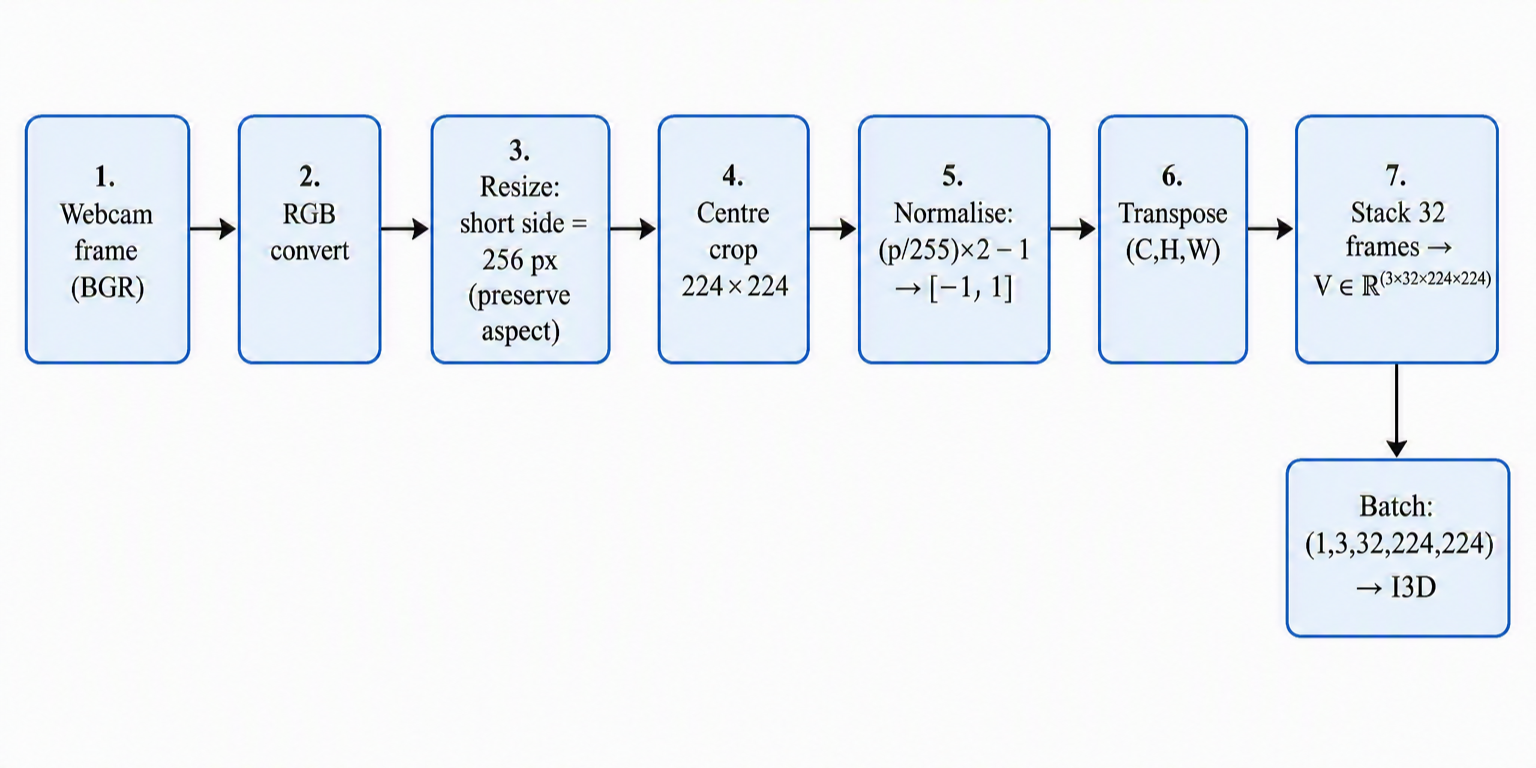
\includegraphics[width=0.95\textwidth]{images/fig_4-1_asl_rgb_preprocess.png}
\caption{ASL word RGB clip preprocessing (Model~3). Each frame passes through colour conversion, aspect-preserving resize (short side 256\,px), centre crop $224\!\times\!224$, $[-1,1]$ normalisation, and $(C,H,W)$ transpose before accumulation in a 32-frame deque (Table~\ref{tab:ch4-asl-preproc}, Equations~\eqref{eq:ch4-resize}--\eqref{eq:ch4-clip}).}
\label{fig:ch4-asl-preprocess}
\end{figure}
\vspace{0.6cm}
\clearpage
% --- 4.3 MODEL 3: INCEPTION I3D ---
\noindent\textbf{4.3\quad MODEL 3 --- ASL WORD INCEPTION I3D}\par
\addcontentsline{toc}{section}{\numberline{4.3}MODEL 3 --- ASL WORD INCEPTION I3D}
\vspace{0.4cm}

\noindent\textbf{Problem.} ASL word meaning depends on hand shape, arm trajectory, and whole-body motion across roughly one second of video. A per-frame landmark vector cannot capture the spatio-temporal dynamics that distinguish glosses with similar handshapes but different movement paths~\cite{li2020wlasl}.\par\vspace{0.4cm}

\noindent\textbf{4.3.1\quad Architectural Family --- Inflated 3-D ConvNet:}\par
\addcontentsline{toc}{subsection}{\numberline{4.3.1}Architectural Family --- Inflated 3-D ConvNet:}
\vspace{0.3cm}

\noindent Inception I3D (Carreira \& Zisserman, 2017) extends the Inception-v1 image backbone by replacing every 2-D convolution filter $k_h \times k_w$ with a volumetric filter $k_t \times k_h \times k_w$ that operates jointly over time and space~\cite{li2020wlasl}. The ``inflation'' initialisation bootstraps 3-D weights from pretrained 2-D ImageNet weights by replicating each filter along the temporal axis and dividing by $k_t$:
\begin{equation}
W^{3\text{D}}_{:,:,\,t,:,:} = \frac{W^{2\text{D}}}{k_t}, \qquad t = 1,\ldots,k_t,
\label{eq:ch4-inflate}
\end{equation}
so that the initial response to a static frame matches the 2-D pretrained response. This allows the model to start from spatially rich ImageNet features and adapt to motion during fine-tuning on video data.\par\vspace{0.3cm}

\noindent\textbf{4.3.2\quad Building Block --- Unit3D:}\par
\addcontentsline{toc}{subsection}{\numberline{4.3.2}Building Block --- Unit3D:}
\vspace{0.3cm}

\noindent Every convolutional stage is implemented as a \textbf{Unit3D} block: a 3-D convolution with dynamically computed SAME padding, followed by Batch Normalisation and ReLU. For a feature volume $\mathbf{A} \in \mathbb{R}^{N \times C_{\text{in}} \times T' \times H' \times W'}$ and filter bank $\mathbf{F} \in \mathbb{R}^{C_{\text{out}} \times C_{\text{in}} \times k_t \times k_h \times k_w}$:
\begin{equation}
(\mathbf{A} \!\ast\! \mathbf{F})_{n,c,t,h,w} = \sum_{c'} \sum_{\delta_t} \sum_{\delta_h} \sum_{\delta_w} \mathbf{A}_{n,c',\,t+\delta_t,\,h+\delta_h,\,w+\delta_w} \cdot \mathbf{F}_{c,c',\,\delta_t,\delta_h,\delta_w}.
\label{eq:ch4-3dconv}
\end{equation}
Batch Normalisation~\cite{ioffe2015batchnorm} stabilises activations across the training batch:
\begin{equation}
\mathbf{Z} = \mathrm{ReLU}\!\left(\gamma\,\frac{\mathbf{A}\!\ast\!\mathbf{F} - \mu_B}{\sqrt{\sigma_B^2 + \varepsilon}} + \beta\right), \qquad \varepsilon = 10^{-3},
\label{eq:ch4-bn}
\end{equation}
where $\mu_B, \sigma_B^2$ are the per-channel batch mean and variance, and $\gamma, \beta$ are learned scale and shift parameters ($\varepsilon = 10^{-3}$).\par\vspace{0.3cm}
\clearpage
\noindent\textbf{4.3.3\quad InceptionModule --- 4-Branch Parallel Block:}\par
\addcontentsline{toc}{subsection}{\numberline{4.3.3}InceptionModule --- 4-Branch Parallel Block:}
\vspace{0.3cm}

\noindent Each Inception stage runs four branches in parallel and channel-concatenates their outputs. For input $\mathbf{A}$ with $C_{\text{in}}$ channels and branch output sizes $[n_0, n_{1a}, n_{1b}, n_{2a}, n_{2b}, n_{3b}]$:
\begin{align}
\text{Branch~0 (direct):}\quad & \mathbf{B}_0 = \mathrm{Unit3D}(\mathbf{A};\;1\!\times\!1\!\times\!1,\;n_0), \label{eq:ch4-b0} \\
\text{Branch~1 (bottleneck+3$\times$3):}\quad & \mathbf{B}_1 = \mathrm{Unit3D}\!\bigl(\mathrm{Unit3D}(\mathbf{A};\;1\!\times\!1\!\times\!1,\;n_{1a});\;3\!\times\!3\!\times\!3,\;n_{1b}\bigr), \label{eq:ch4-b1} \\
\text{Branch~2 (bottleneck+3$\times$3):}\quad & \mathbf{B}_2 = \mathrm{Unit3D}\!\bigl(\mathrm{Unit3D}(\mathbf{A};\;1\!\times\!1\!\times\!1,\;n_{2a});\;3\!\times\!3\!\times\!3,\;n_{2b}\bigr), \label{eq:ch4-b2} \\
\text{Branch~3 (pool+project):}\quad & \mathbf{B}_3 = \mathrm{Unit3D}\!\bigl(\mathrm{MaxPool}_{3\times3\times3}(\mathbf{A});\;1\!\times\!1\!\times\!1,\;n_{3b}\bigr). \label{eq:ch4-b3}
\end{align}
\begin{equation}
\mathrm{InceptionModule}(\mathbf{A}) = \mathrm{Concat}(\mathbf{B}_0, \mathbf{B}_1, \mathbf{B}_2, \mathbf{B}_3) \in \mathbb{R}^{N \times (n_0 + n_{1b} + n_{2b} + n_{3b}) \times T' \times H' \times W'}.
\label{eq:ch4-incept}
\end{equation}
The $1\!\times\!1\!\times\!1$ bottlenecks in Branches~1--3 reduce channel depth before the more expensive $3\!\times\!3\!\times\!3$ convolutions, capturing multi-scale context efficiently. Branch~3 uses max-pooling followed by a $1\!\times\!1\!\times\!1$ projection, providing a pooling path without additional 3-D convolution cost.\par\vspace{0.4cm}

\begin{figure}[H]
\centering
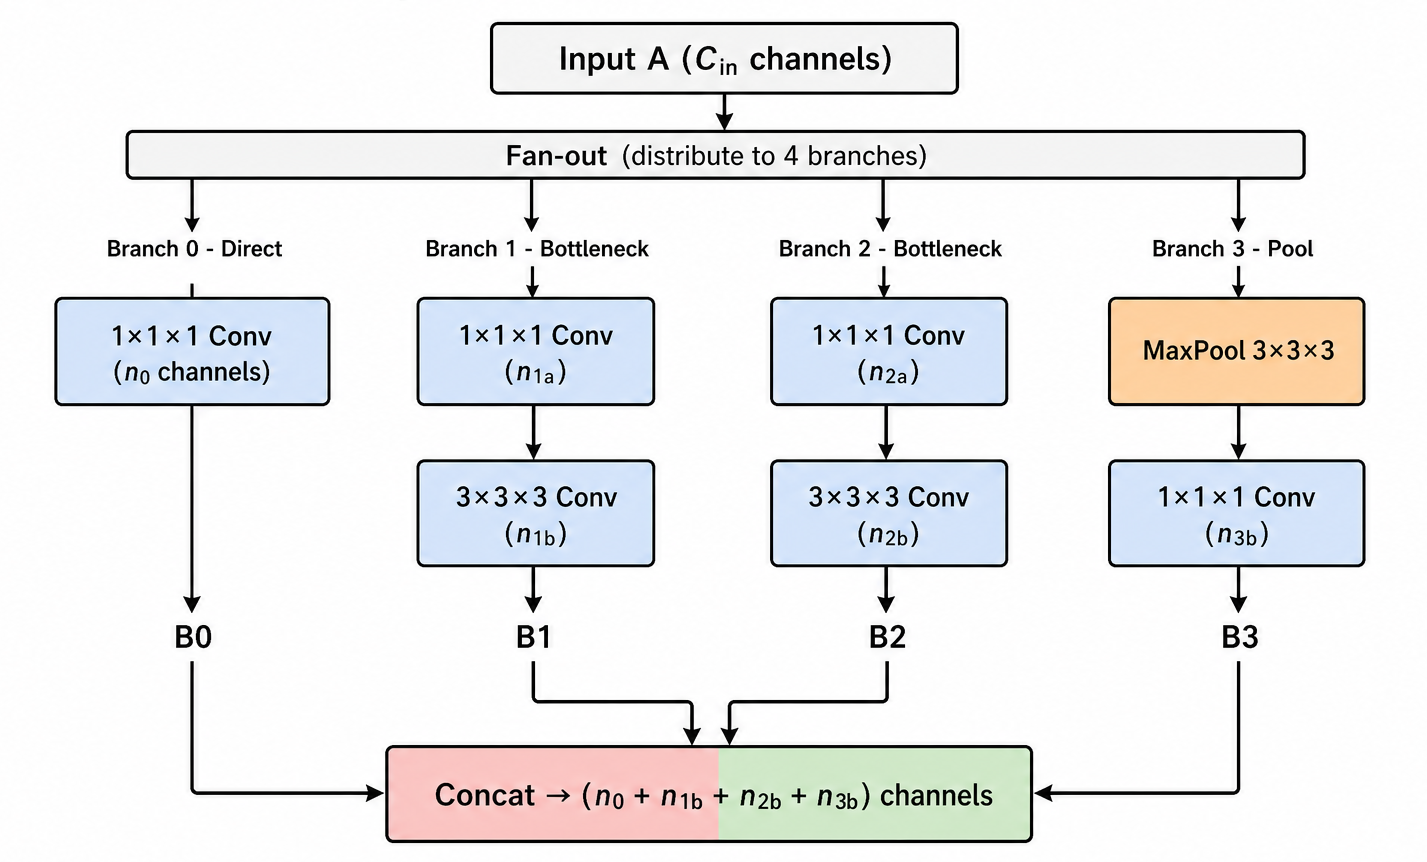
\includegraphics[width=0.99\textwidth]{images/fig_4-9_inception_module.png}
\caption{InceptionModule 4-branch parallel structure (Equations~\eqref{eq:ch4-b0}--\eqref{eq:ch4-incept}). All branches process the same input $\mathbf{A}$ simultaneously; outputs are channel-concatenated. Example for \texttt{Mixed\_3b}: $[64, 96, 128, 16, 32, 32] \rightarrow 64+128+32+32 = 256$ output channels.}
\label{fig:ch4-inception-branches}
\end{figure}
\vspace{0.4cm}

\noindent\textbf{4.3.4\quad Full Layer Stack:}\par
\addcontentsline{toc}{subsection}{\numberline{4.3.4}Full Layer Stack:}
\vspace{0.3cm}

\noindent Table~\ref{tab:ch4-i3d-stack} lists every stage in order for Model~3. The input enters as $\hat{\mathbf{V}} \in \mathbb{R}^{1 \times 3 \times 32 \times 224 \times 224}$.

\begin{table}[H]
\centering
\caption{Inception I3D layer stack (Model~3, ASL words). Branch configs for Inception stages: $[n_0, n_{1a}, n_{1b}, n_{2a}, n_{2b}, n_{3b}]$ per Equation~\eqref{eq:ch4-incept}. Input: $(1, 3, 32, 224, 224)$.}
\label{tab:ch4-i3d-stack}
\footnotesize
\renewcommand{\arraystretch}{1.6} % Adds vertical padding so the text doesn't hit the borders
\resizebox{\textwidth}{!}{%
\begin{tabular}{|c|l|l|c|l|}
\hline
\textbf{\#} & \textbf{Stage name} & \textbf{Layer type} & \textbf{Out ch.} & \textbf{Config / notes} \\ \hline
1 & Conv3d\_1a\_7x7 & Unit3D & 64 & kernel $7\!\times\!7\!\times\!7$, stride $(2,2,2)$, padding $3$ \\ \hline
2 & MaxPool3d\_2a\_3x3 & MaxPool3d (SAME) & 64 & kernel $(1,3,3)$, stride $(1,2,2)$ \\ \hline
3 & Conv3d\_2b\_1x1 & Unit3D & 64 & kernel $1\!\times\!1\!\times\!1$ \\ \hline
4 & Conv3d\_2c\_3x3 & Unit3D & 192 & kernel $3\!\times\!3\!\times\!3$ \\ \hline
5 & MaxPool3d\_3a\_3x3 & MaxPool3d (SAME) & 192 & kernel $(1,3,3)$, stride $(1,2,2)$ \\ \hline
6 & Mixed\_3b & InceptionModule & 256 & $[64,\;96,\;128,\;16,\;32,\;32]$ \\ \hline
7 & Mixed\_3c & InceptionModule & 480 & $[128,\;128,\;192,\;32,\;96,\;64]$ \\ \hline
8 & MaxPool3d\_4a\_3x3 & MaxPool3d (SAME) & 480 & kernel $(3,3,3)$, stride $(2,2,2)$ \\ \hline
9 & Mixed\_4b & InceptionModule & 512 & $[192,\;96,\;208,\;16,\;48,\;64]$ \\ \hline
10 & Mixed\_4c & InceptionModule & 512 & $[160,\;112,\;224,\;24,\;64,\;64]$ \\ \hline
11 & Mixed\_4d & InceptionModule & 512 & $[128,\;128,\;256,\;24,\;64,\;64]$ \\ \hline
12 & Mixed\_4e & InceptionModule & 528 & $[112,\;144,\;288,\;32,\;64,\;64]$ \\ \hline
13 & Mixed\_4f & InceptionModule & 832 & $[256,\;160,\;320,\;32,\;128,\;128]$ \\ \hline
14 & MaxPool3d\_5a\_2x2 & MaxPool3d & 832 & kernel $(2,2,2)$, stride $(2,2,2)$ \\ \hline
15 & Mixed\_5b & InceptionModule & 832 & $[256,\;160,\;320,\;32,\;128,\;128]$ \\ \hline
16 & Mixed\_5c & InceptionModule & 1024 & $[384,\;192,\;384,\;48,\;128,\;128]$ \\ \hline
17 & AvgPool3d & nn.AvgPool3d & 1024 & kernel $(2,7,7)$, stride $(1,1,1)$ \\ \hline
18 & Dropout & nn.Dropout & 1024 & $p = 0.5$ \\ \hline
19 & Logits (Unit3D) & 3-D conv & \textbf{100} & $1\!\times\!1\!\times\!1$, no BN, no activation, bias=True \\ \hline
\end{tabular}%
}
\end{table}
\vspace{0.4cm}

\begin{figure}[H]
\centering
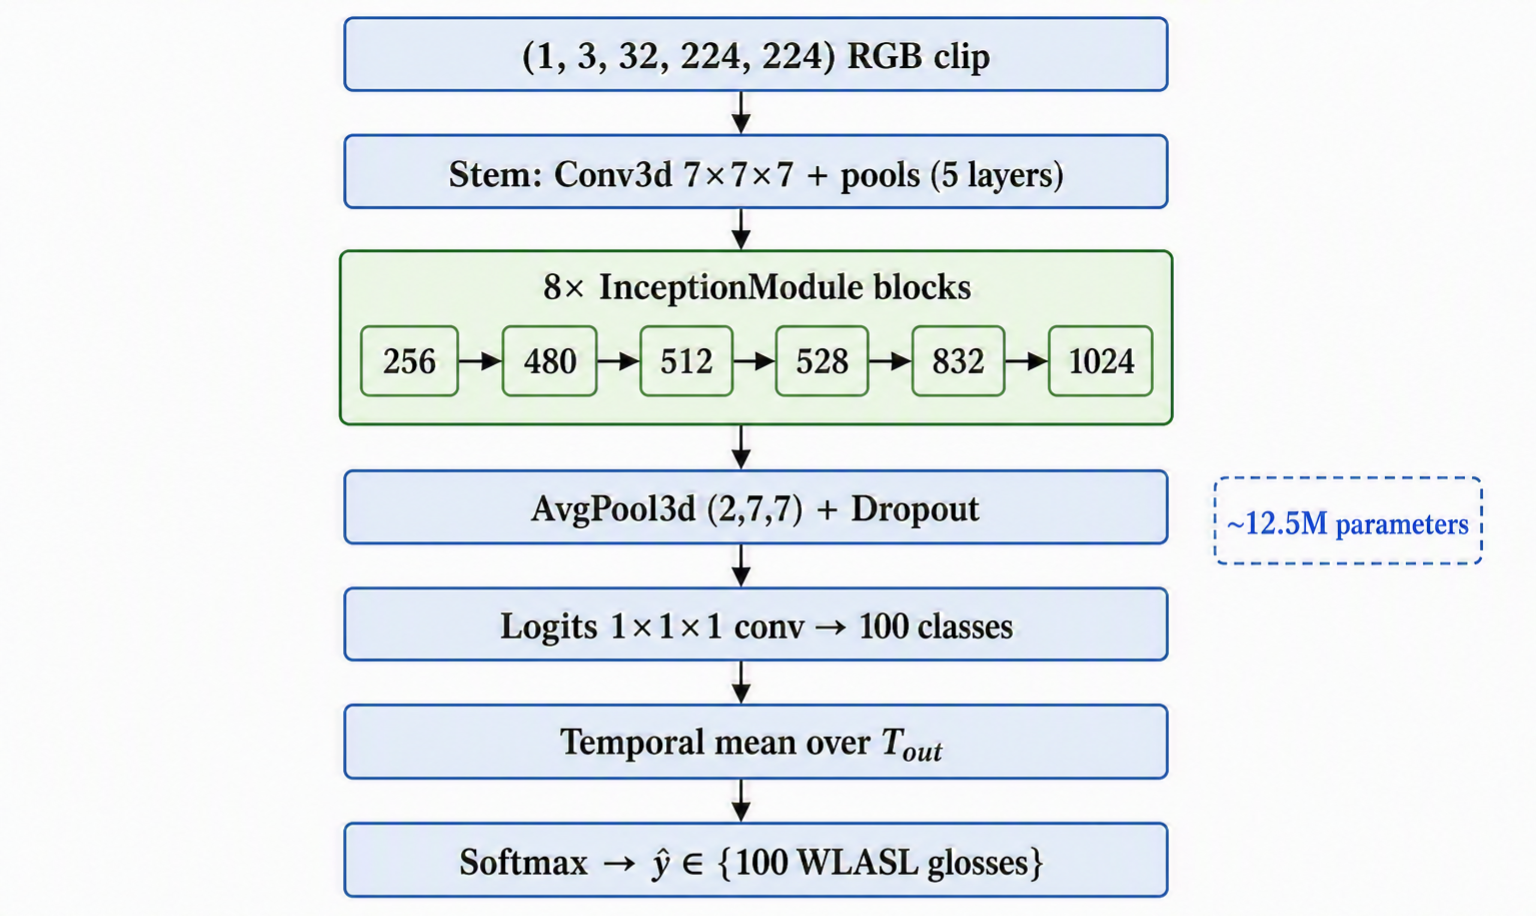
\includegraphics[width=0.99\textwidth]{images/fig_4-2_i3d_forward_pass.png}
\caption{Inception I3D forward pass (Model~3). The $(1,3,32,224,224)$ clip passes through the stem, eight Inception modules (Table~\ref{tab:ch4-i3d-stack}), AvgPool, dropout, and a 100-way logit head; logits are temporally averaged before softmax (Equations~\eqref{eq:ch4-temporal-mean}--\eqref{eq:ch4-i3d-softmax}).}
\label{fig:ch4-i3d-flow}
\end{figure}
\vspace{0.4cm}

\noindent\textbf{4.3.5\quad Temporal Logit Aggregation and Softmax:}\par
\addcontentsline{toc}{subsection}{\numberline{4.3.5}Temporal Logit Aggregation and Softmax:}
\vspace{0.3cm}

\noindent After the forward pass, the logit layer produces a tensor $\mathbf{L} \in \mathbb{R}^{1 \times 100 \times T_{\text{out}}}$ (residual temporal dimension after AvgPool). The spatial dimensions have already been squeezed. Logits are averaged across the residual time axis before softmax:
\begin{equation}
\bar{\mathbf{z}} = \frac{1}{T_{\text{out}}} \sum_{\tau=1}^{T_{\text{out}}} \mathbf{L}_{0,:,\,\tau} \in \mathbb{R}^{100},
\label{eq:ch4-temporal-mean}
\end{equation}
\begin{equation}
P(y{=}k \mid \hat{\mathbf{V}}) = \frac{\exp(\bar{z}_k)}{\displaystyle\sum_{j=1}^{100} \exp(\bar{z}_j)}, \qquad \hat{y} = \arg\max_k P(y{=}k \mid \hat{\mathbf{V}}).
\label{eq:ch4-i3d-softmax}
\end{equation}
Averaging logits before softmax (late temporal fusion on logit space) is numerically more calibrated than averaging softmax probabilities independently~\cite{li2020wlasl}.\par\vspace{0.3cm}
\clearpage
\noindent\textbf{4.3.6\quad Checkpoint and Parameter Count:}\par
\addcontentsline{toc}{subsection}{\numberline{4.3.6}Checkpoint and Parameter Count:}
\vspace{0.3cm}

\noindent Model~3 is initialised as Inception I3D with a 400-class Kinetics head, the logit layer is replaced for $C{=}100$ WLASL glosses, and pretrained weights are loaded from \texttt{asl\_word\_i3d.pt}. At inference, batch normalisation running statistics are frozen and dropout is disabled.\par\vspace{0.2cm}

\noindent\textbf{Parameter count.} The Kinetics-400 backbone contributes $\sim$12.7\,M parameters; replacing the 400-class head ($1024 \times 400 + 400 = 409\,600$ params) with a 100-class head ($1024 \times 100 + 100 = 102\,500$ params) reduces the total by $\sim$307\,K, giving approximately \textbf{12.5 million} parameters for Model~3.\par\vspace{0.6cm}

% --- 4.4 ASL STABILISATION ---
\noindent\textbf{4.4\quad ASL WORD STABILISATION DECODER}\par
\addcontentsline{toc}{section}{\numberline{4.4}ASL WORD STABILISATION DECODER}
\vspace{0.4cm}

\noindent Per-clip I3D predictions can be noisy if a signing motion is captured mid-gesture or the frame buffer transitions between two words. Eshara's \textbf{ASL word stabilisation decoder} suppresses premature or repeated commits using three jointly-evaluated conditions (Table~\ref{tab:ch4-stab-params}):\par\vspace{0.3cm}

\begin{table}[H]
\centering
\caption{ASL word stabilisation parameters (Model~3).}
\label{tab:ch4-stab-params}
\small
\renewcommand{\arraystretch}{1.6}% Adds vertical padding so the text doesn't hit the borders
\begin{tabular}{|P{4.0cm}|c|P{7.2cm}|}
\hline
\textbf{Parameter} & \textbf{Value} & \textbf{Role} \\ \hline
\texttt{FRAME\_BUFFER\_SIZE} & 32 & Frames buffered per inference call \\ \hline
\texttt{STAB\_WINDOW} & 10 & Recent predictions evaluated for voting \\ \hline
\texttt{STAB\_THRESH} & 6 & Minimum matching predictions to consider committing \\ \hline
\texttt{MIN\_CONFIDENCE} & 0.50 & Minimum softmax probability to accept a prediction \\ \hline
\texttt{HOLD\_COOLDOWN} & 1.2\,s & Lock-out period after any commit \\ \hline
Repeat cooldown & 2.4\,s & Lock-out for committing the same word twice \\ \hline
\end{tabular}
\end{table}
\vspace{0.4cm}

\noindent A word is committed when \textbf{all} three conditions simultaneously hold:
\begin{enumerate}
\item \textbf{Majority agreement:} the mode of the last 10 predictions appears $\geq 6$ times.
\item \textbf{Confidence gate:} $\max_k P(y{=}k \mid \hat{\mathbf{V}}) \geq 0.50$.
\item \textbf{Cooldown gate:} $t_{\text{now}} - t_{\text{last\_commit}} > 1.2$\,s (or $> 2.4$\,s for the same word).
\end{enumerate}
On commit, both the frame deque and prediction window are cleared. The endpoint returns \texttt{\{"status":"committed",\ldots\}} or \texttt{\{"status":"buffering",\ldots\}} between commits (Figure~\ref{fig:ch4-asl-stab}).\par\vspace{0.4cm}
\begin{figure}[H]
\centering
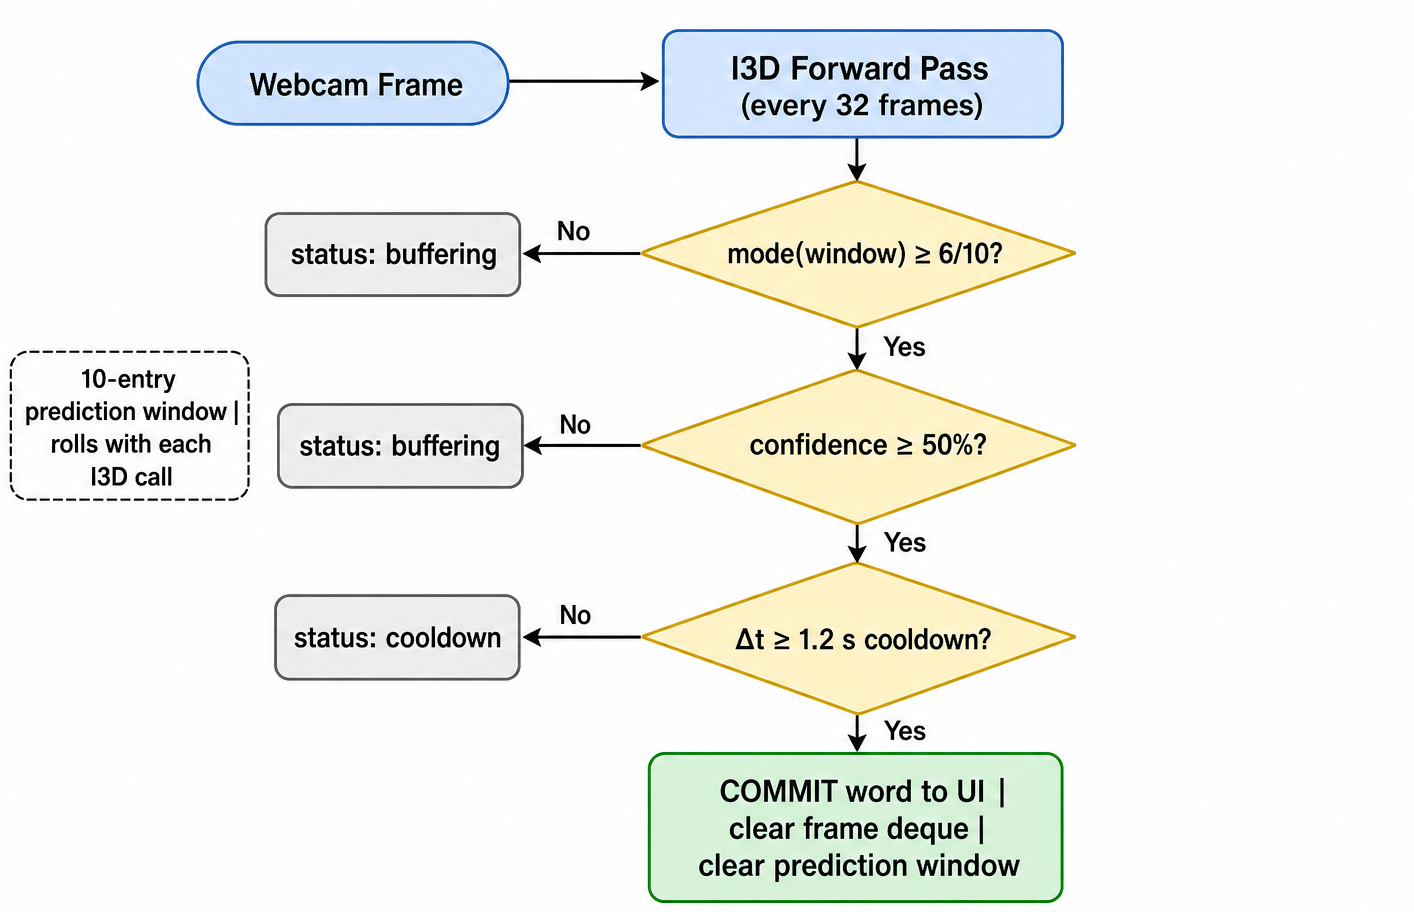
\includegraphics[width=0.82\textwidth]{images/fig_4-8_asl_word_stabiliser.png}
\caption{ASL word stabilisation decoder (Model~3). Three gates --- majority vote (6/10), confidence ($\geq$50\,\%), and cooldown ($\geq$1.2\,s) --- must pass before a gloss is committed (Table~\ref{tab:ch4-stab-params}).}
\label{fig:ch4-asl-stab}
\end{figure}
\vspace{0.2cm} % Cramped from 0.4cm

% --- 4.5 ASL INFERENCE PATH ---
\noindent\textbf{4.5\quad ASL INFERENCE PATH (End-to-End)}\par
\addcontentsline{toc}{section}{\numberline{4.5}ASL INFERENCE PATH (END-TO-END)}
\vspace{0.2cm} % Cramped from 0.4cm

\noindent The model-side path from a single RGB frame to a committed gloss probability vector is:
\vspace{-0.1cm} % Pulled list closer to intro text

\begin{enumerate}
\setlength{\itemsep}{0pt} % Cramped list spacing
\setlength{\parskip}{0pt}
\item Each incoming frame is preprocessed via Steps 1--5 of Table~\ref{tab:ch4-asl-preproc} and appended to a 32-frame rolling buffer.
\item When the buffer is full, frames are stacked to $\mathbf{V} \in \mathbb{R}^{3 \times 32 \times 224 \times 224}$ and batched as $(1,3,32,224,224)$.
\item The I3D forward pass (Equations~\eqref{eq:ch4-3dconv}--\eqref{eq:ch4-i3d-softmax}) returns logits; temporal averaging and softmax produce a 100-D probability vector.
\item The stabilisation decoder (Section~4.4) gates whether a gloss is committed to the UI.
\end{enumerate}
\vspace{0.2cm} % Cramped from 0.3cm

\enlargethispage{\baselineskip} % Extends page bottom margin by 1 line to catch spilling text

\noindent HTTP routing, session management, and the React sentence panel are described in Chapter~5.\par\vspace{0.15cm} % Cramped from 0.3cm

\noindent\textbf{Artifacts.} See Table~\ref{tab:ch4-artifacts} (Model~3 row). Results are reported in Chapter~6.\par\vspace{0.3cm} % Cramped from 0.6cm
% ==========================================================
% PART B: ArSL WORD RECOGNITION
% ==========================================================
\newpage
\vspace*{-0.2cm} % Pulls the title up slightly into the top margin
\begin{center}
\large\textbf{PART B: ArSL WORD RECOGNITION (Model~4 --- Stacked BiLSTM)}
\end{center}
\addcontentsline{toc}{section}{\textbf{PART B: ArSL WORD RECOGNITION (Model 4)}}
\vspace{0.2cm} % Cramped from 0.4cm
\noindent\rule{\textwidth}{0.8pt}
\vspace{0.2cm} % Cramped from 0.4cm

% --- 4.6 KARSL DATASET ---
\noindent\textbf{4.6\quad KArSL DATASET AND SPLIT POLICY}\par
\addcontentsline{toc}{section}{\numberline{4.6}KArSL DATASET AND SPLIT POLICY}
\vspace{0.2cm} % Cramped from 0.4cm

\noindent KArSL-502 (Sidig et al., 2021) is the primary large-scale Arabic sign-language video corpus, containing $\sim$24\,000 clips across 502 sign IDs recorded by three signers under controlled studio conditions~\cite{sidig2021karsl,karslgithub2021}. Table~\ref{tab:ch4-karsl-stats} summarises the subset used for the graduation ArSL word model.\par\vspace{0.2cm} % Cramped from 0.4cm

\begin{table}[H]
\centering
\caption{KArSL dataset statistics for the Model~4 (ArSL word) graduation deployment.}
\label{tab:ch4-karsl-stats}
\footnotesize % Shrunk from \small to save space
\renewcommand{\arraystretch}{1.7} % Reduced from 1.6 to tighten the rows
\begin{tabular}{|P{4.0cm}|P{8.0cm}|}
\hline
\textbf{Property} & \textbf{Value} \\ \hline
Full corpus & KArSL-502: $\sim$24\,000 clips, 502 sign IDs \\ \hline
Sign taxonomy & Numbers 1--31, letters 32--70, \textbf{words 71--502} \\ \hline
Graduation subset & \textbf{100 Arabic word classes (SignID 71--170)} \\ \hline
Avg.\ clips / class & $\sim$50--60 (3 signers $\times$ $\sim$20 repetitions) \\ \hline
Signers & 3 (Arab Saudi dialect) \\ \hline
Clip length (raw) & Variable; clipped or padded to 48 frames \\ \hline
Feature dim & 225-D (Pose 99-D + left hand 63-D + right hand 63-D) \\ \hline
Normalisation & Nose-centred pose; wrist-centred per hand \\ \hline
Test split & Held-out signer partition (not used in training) \\ \hline
Label source & \texttt{KARSL-502\_\allowbreak Labels.xlsx} rows 71--170 \\ \hline
Test Top-1 & \textbf{99.62\,\%} (encoded in checkpoint filename) \\ \hline
\end{tabular}
\end{table}
\vspace{0.2cm} % Cramped from 0.4cm

\noindent The vocabulary is restricted to SignID 71--170 (body and medical Arabic words) rather than the full 502-class corpus to maintain approximately 50 training samples per class --- above the threshold at which the BiLSTM generalises reliably without overfitting to the three-signer studio distribution~\cite{sidig2021karsl}.\par\vspace{0.3cm} % Cramped from 0.6cm

% --- 4.7 ArSL FEATURE EXTRACTION ---
\noindent\textbf{4.7\quad ArSL FEATURE EXTRACTION --- 225-D HOLISTIC PIPELINE}\par
\addcontentsline{toc}{section}{\numberline{4.7}ArSL FEATURE EXTRACTION --- 225-D HOLISTIC PIPELINE}
\vspace{0.4cm}

\noindent Unlike I3D, the ArSL model operates on \textbf{body-relative landmark coordinates} extracted by MediaPipe Holistic. This representation decouples the classification problem from signer size and camera distance, and reduces the input dimensionality by orders of magnitude compared with raw pixels~\cite{zhang2020mediapipe}. Instead of passing heavy image tensors through convolutional layers, the system tracks the skeletal geometry directly over time, making it highly efficient for web deployment.\par\vspace{0.4cm}

\noindent\textbf{4.7.1\quad 225-D Feature Vector Composition:}\par
\addcontentsline{toc}{subsection}{\numberline{4.7.1}225-D Feature Vector Composition:}
\vspace{0.3cm}

\noindent The 225-D feature vector concatenates three distinct spatial blocks. Notably, the dense 468-point face mesh provided by the default MediaPipe Holistic API is entirely excluded. Omitting detailed facial geometry prevents the model from overfitting to specific signer identities while drastically reducing the computational payload per frame. Broad non-manual grammatical markers, such as head tilts or torso shifts, are already adequately captured by the core pose skeleton. The final vector comprises exactly $33{\times}3 + 21{\times}3 + 21{\times}3 = 225$ spatial coordinates:\par\vspace{0.3cm}

\begin{table}[H]
\centering
\caption{225-D Holistic feature-vector block decomposition (ArSL word model). Missing detections are zero-filled.}
\label{tab:ch4-holistic-blocks}
\small
\renewcommand{\arraystretch}{1.4} % Adds vertical padding so the text doesn't hit the borders
\begin{tabular}{|c|P{2.0cm}|P{2.0cm}|c|P{5.6cm}|}
\hline
\textbf{Block} & \textbf{Source} & \textbf{Landmarks} & \textbf{Dim} & \textbf{Reference (subtracted)} \\ \hline
Pose & MediaPipe Pose & 33 $\times$ $(x,y,z)$ & 99 & Nose (landmark 0): $\mathbf{p}_0^{\text{pose}}$ \\ \hline
Left hand & MediaPipe Hands & 21 $\times$ $(x,y,z)$ & 63 & Left wrist (landmark 0): $\mathbf{q}_0^{\text{lh}}$ \\ \hline
Right hand & MediaPipe Hands & 21 $\times$ $(x,y,z)$ & 63 & Right wrist (landmark 0): $\mathbf{q}_0^{\text{rh}}$ \\ \hline
\textbf{Total} & --- & --- & \textbf{225} & Concatenated body-relative vector \\ \hline
\end{tabular}
\end{table}
\vspace{0.4cm}
\clearpage
\noindent\textbf{Local Coordinate Normalisation.} Raw $(x, y, z)$ values from the webcam fluctuate wildly depending on where the user stands in the frame. To make the features translation-invariant, each anatomical block is shifted to a local origin. The pose landmarks are centered by subtracting the nose coordinates ($\mathbf{p}_0^{\text{pose}}$) from all upper-body joints. Similarly, each hand is independently centered by subtracting its respective wrist coordinates ($\mathbf{q}_0^{\text{lh}}$ and $\mathbf{q}_0^{\text{rh}}$). This ensures that a specific handshape feature vector remains mathematically identical whether the user signs it near their chest or high above their head.\par\vspace{0.3cm}

\noindent\textbf{Handling Occlusion.} Fast signing often causes motion blur, hand-over-hand occlusion, or frames where the hands exit the camera view. In these instances, the missing blocks are explicitly zero-filled rather than linearly interpolated. Because the features are mean-centered at zero (the wrist or nose), passing a vector of zeros acts as a mathematically neutral signal to the BiLSTM, preventing erratic spatial jumping or noisy artifacts in the sequence data.\par\vspace{0.4cm}
\begin{figure}[H]
\centering
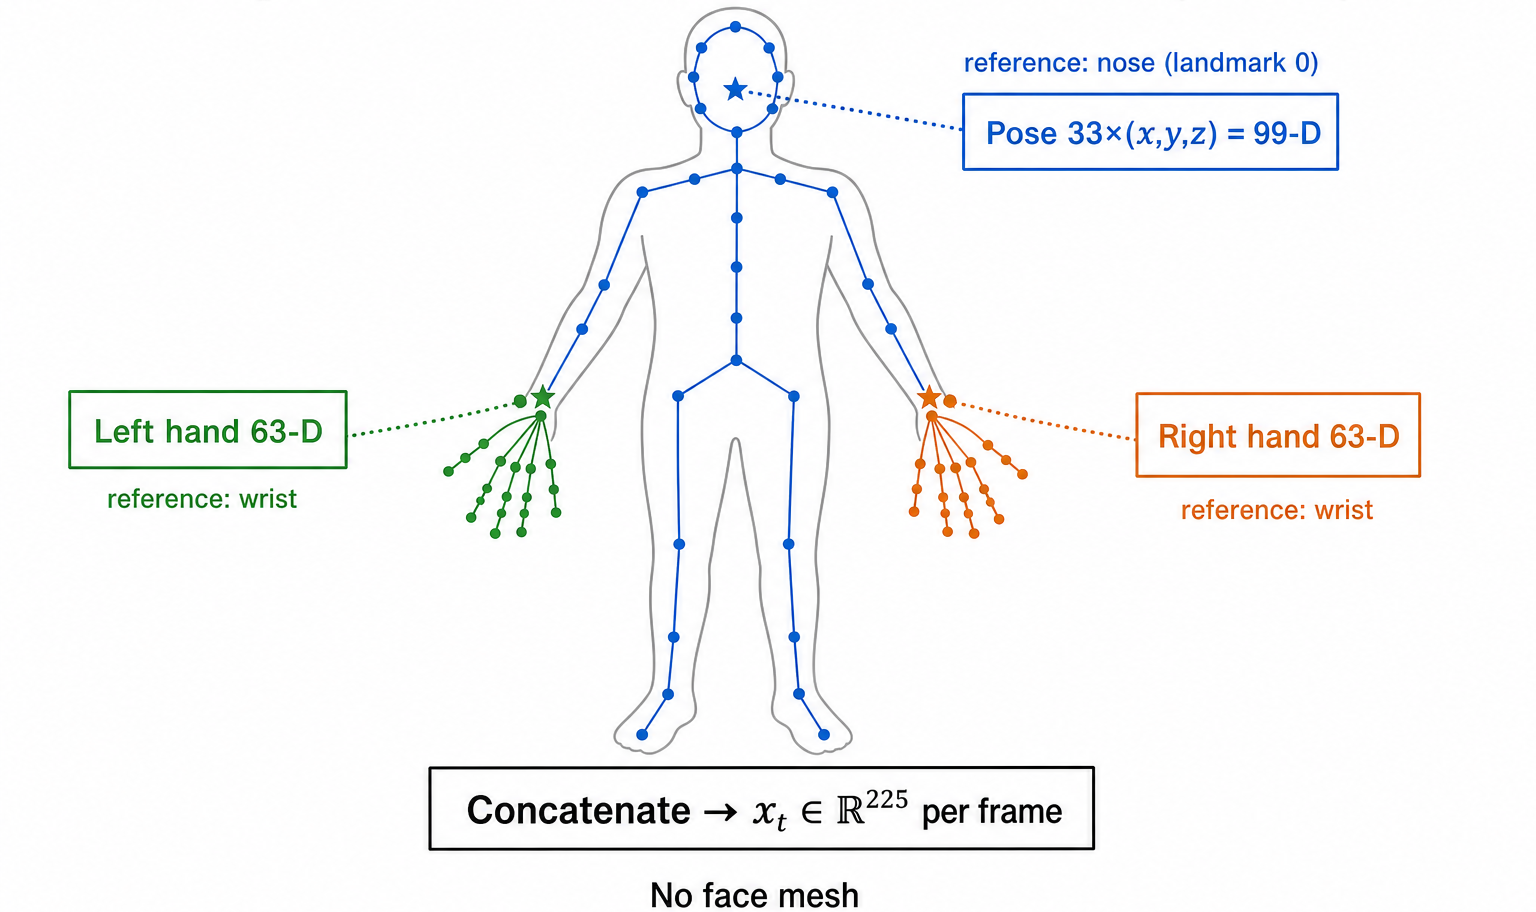
\includegraphics[width=0.99\textwidth]{images/fig_4-4_arsl_holistic_225d.png}
\caption{225-D Holistic feature topology for ArSL words (Model~4). Pose (99-D) is nose-centred; each hand block (63-D) is wrist-centred. No face mesh is included (Table~\ref{tab:ch4-holistic-blocks}).}
\label{fig:ch4-holistic-topology}
\end{figure}
\vspace{0.4cm}

\begin{figure}[H]
\centering
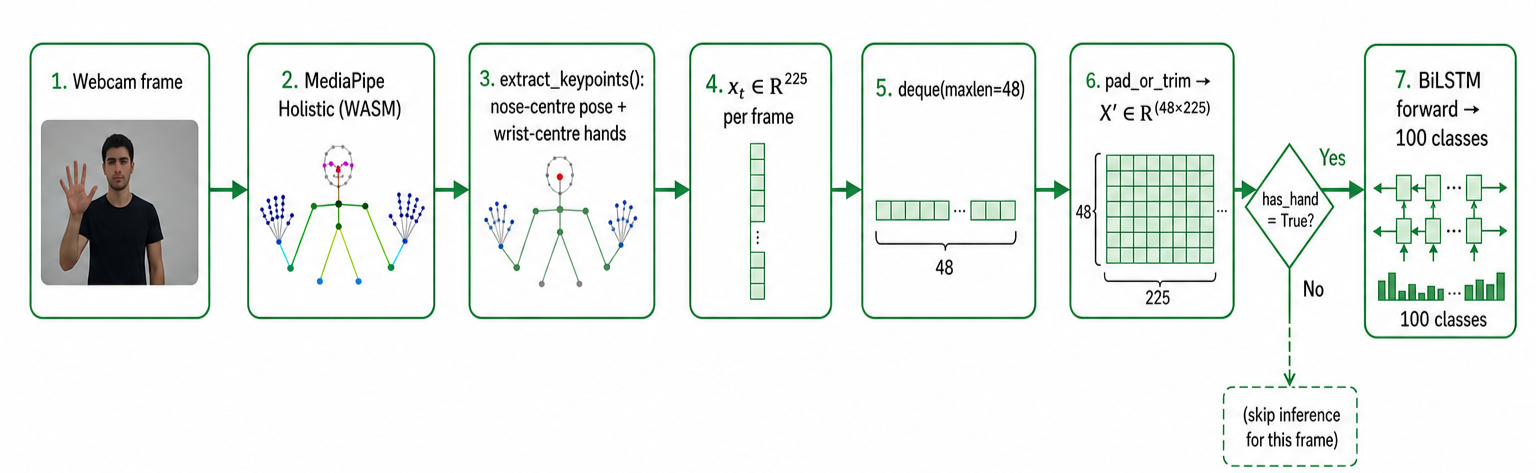
\includegraphics[width=0.99\textwidth]{images/fig_4-5_arsl_holistic_pipeline.png}
\caption{ArSL word Holistic extraction pipeline (Model~4). Landmarks are normalised per frame, buffered to 48 frames, aligned via trim/pad, and classified by the stacked BiLSTM when \texttt{has\_hand} is true (Sections~4.7--4.9).}
\label{fig:ch4-arsl-pipeline}
\end{figure}
\vspace{0.4cm}

\noindent\textbf{4.7.2\quad Body-Relative Normalisation (adjust\_landmarks):}\par
\addcontentsline{toc}{subsection}{\numberline{4.7.2}Body-Relative Normalisation:}
\vspace{0.3cm}

\noindent Each landmark block is centred on a reference joint by subtracting the anchor point $\mathbf{p}_0$ from every $(x,y,z)$ triplet, making the block translation-invariant:
\begin{equation}
\hat{\mathbf{p}}_i^{\text{pose}} = \mathbf{p}_i^{\text{pose}} - \underbrace{\mathbf{p}_0^{\text{pose}}}_{\text{nose}}, \quad i = 0,\ldots,32,
\label{eq:ch4-adjust-pose}
\end{equation}
\begin{equation}
\hat{\mathbf{q}}_j^{\text{hand}} = \mathbf{q}_j^{\text{hand}} - \underbrace{\mathbf{q}_0^{\text{hand}}}_{\text{wrist}}, \quad j = 0,\ldots,20, \quad \text{(left and right hands independently).}
\label{eq:ch4-adjust-hand}
\end{equation}
The three adjusted blocks are flattened and concatenated to form the per-frame feature vector:
\begin{equation}
\mathbf{x}_t = \bigl[\hat{\mathbf{p}}^{\text{pose}}_t;\;\hat{\mathbf{q}}^{\text{lh}}_t;\;\hat{\mathbf{q}}^{\text{rh}}_t\bigr] \in \mathbb{R}^{225}.
\label{eq:ch4-holvec}
\end{equation}
If no pose is detected, $\hat{\mathbf{p}}^{\text{pose}}_t = \mathbf{0}_{99}$; if a hand is absent, the corresponding 63-D block is $\mathbf{0}_{63}$. The live client applies the same zero-fill convention during inference.\par\vspace{0.4cm}

\noindent\textbf{4.7.3\quad Clip Alignment (Trim / Pad):}\par
\addcontentsline{toc}{subsection}{\numberline{4.7.3}Clip Alignment (Trim / Pad):}
\vspace{0.3cm}

\noindent KArSL clip durations vary. Model~4 aligns every sequence to exactly $F{=}48$ frames using trim/pad (Equation~\eqref{eq:ch4-padtrim}):
\begin{equation}
\mathbf{X}' = \begin{cases}
\mathbf{X}[0:48, :] & T_{\text{raw}} \geq 48 \quad\text{(take first 48 frames)}, \\[4pt]
\Bigl[\mathbf{X};\;\underbrace{\mathbf{x}_{T_{\text{raw}}},\ldots,\mathbf{x}_{T_{\text{raw}}}}_{48-T_{\text{raw}}}\Bigr] & T_{\text{raw}} < 48 \quad\text{(repeat last frame)}.
\end{cases}
\label{eq:ch4-padtrim}
\end{equation}
Repeating the final frame retains the end-of-sign body configuration rather than introducing a zero-gap discontinuity. The resulting clip is $\mathbf{X}' \in \mathbb{R}^{48 \times 225}$.\par\vspace{0.4cm}

\begin{figure}[H]
\centering
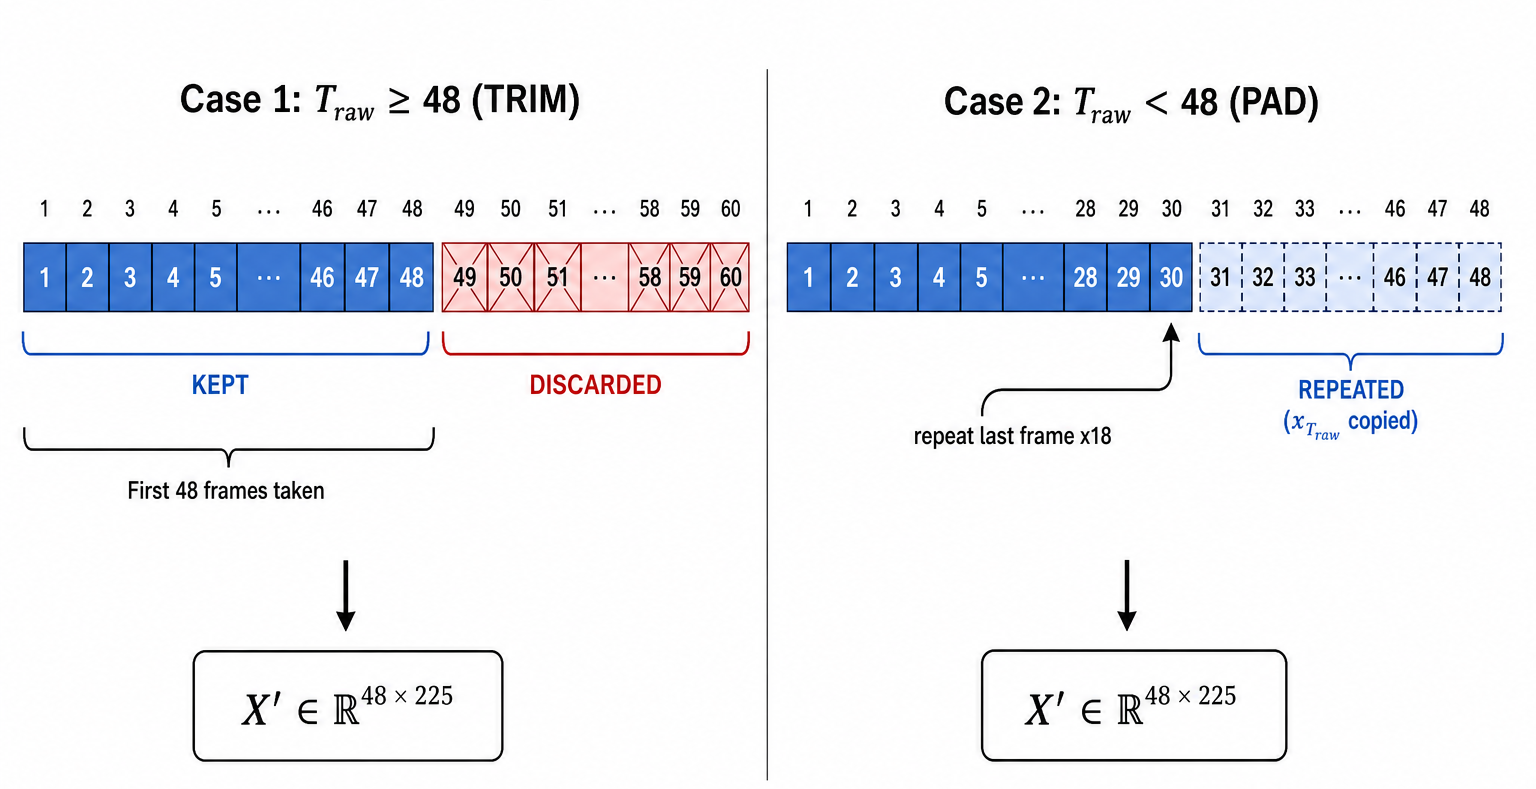
\includegraphics[width=0.99\textwidth]{images/fig_4-10_arsl_padtrim.png}
\caption{Trim/pad clip-alignment policy (Equation~\eqref{eq:ch4-padtrim}). Clips longer than 48 frames are truncated to the first 48; shorter clips are extended by repeating the final body-pose frame until 48 frames are reached. Both cases produce $\mathbf{X}' \in \mathbb{R}^{48 \times 225}$.}
\label{fig:ch4-padtrim}
\end{figure}
\vspace{0.3cm}

\noindent\textbf{No external scaler.} The BiLSTM was trained on raw nose/wrist-centred coordinates (Equations~\eqref{eq:ch4-adjust-pose}--\eqref{eq:ch4-holvec}) without fitting a separate \texttt{StandardScaler}~\cite{pedregosa2011sklearn}. Inference feeds $\mathbf{X}'$ directly into the model without any per-dimension mean/variance correction.\par\vspace{0.6cm}
\clearpage
% --- 4.8 MODEL 4: ArSL BiLSTM ---
\noindent\textbf{4.8\quad MODEL 4 --- ArSL WORD STACKED BiLSTM}\par
\addcontentsline{toc}{section}{\numberline{4.8}MODEL 4 --- ArSL WORD STACKED BiLSTM}
\vspace{0.4cm}

\noindent\textbf{Problem.} Arabic isolated words require two-hand coordination and upper-body motion over 1--2 seconds. The KArSL training set provides only $\sim$50--60 clips per class; a lightweight recurrent model that generalises from compact landmark sequences was therefore preferred over a pixel-intensive 3-D CNN~\cite{sidig2021karsl}.\par\vspace{0.4cm}

\noindent\textbf{4.8.1\quad LSTM Cell Equations:}\par
\addcontentsline{toc}{subsection}{\numberline{4.8.1}LSTM Cell Equations:}
\vspace{0.3cm}

\noindent A single LSTM unit at time step $t$ with input $\mathbf{x}_t \in \mathbb{R}^d$ and previous states $(\mathbf{h}_{t-1}, \mathbf{c}_{t-1}) \in \mathbb{R}^h \times \mathbb{R}^h$ maintains four gated operations~\cite{hochreiter1997long}:
\begin{align}
\mathbf{i}_t &= \sigma(W_i\,\mathbf{x}_t + U_i\,\mathbf{h}_{t-1} + \mathbf{b}_i), \label{eq:ch4-lstm-i} \\
\mathbf{f}_t &= \sigma(W_f\,\mathbf{x}_t + U_f\,\mathbf{h}_{t-1} + \mathbf{b}_f), \label{eq:ch4-lstm-f} \\
\mathbf{o}_t &= \sigma(W_o\,\mathbf{x}_t + U_o\,\mathbf{h}_{t-1} + \mathbf{b}_o), \label{eq:ch4-lstm-o} \\
\tilde{\mathbf{c}}_t &= \tanh(W_c\,\mathbf{x}_t + U_c\,\mathbf{h}_{t-1} + \mathbf{b}_c), \label{eq:ch4-lstm-g} \\
\mathbf{c}_t &= \mathbf{f}_t \odot \mathbf{c}_{t-1} + \mathbf{i}_t \odot \tilde{\mathbf{c}}_t, \label{eq:ch4-lstm-c} \\
\mathbf{h}_t &= \mathbf{o}_t \odot \tanh(\mathbf{c}_t). \label{eq:ch4-lstm-h}
\end{align}
$\sigma$ is sigmoid, $\odot$ is element-wise multiplication. $W_* \in \mathbb{R}^{h \times d}$, $U_* \in \mathbb{R}^{h \times h}$, $\mathbf{b}_* \in \mathbb{R}^h$ are learned parameters. The \textbf{input gate} $\mathbf{i}_t$ writes new content; the \textbf{forget gate} $\mathbf{f}_t$ retains past cell memory; the \textbf{output gate} $\mathbf{o}_t$ exposes the hidden state; the candidate $\tilde{\mathbf{c}}_t$ proposes new cell content. Gating avoids the vanishing-gradient problem over 48-step sequences~\cite{pascanu2013difficulty}.\par\vspace{0.3cm}

\begin{figure}[H]
\centering
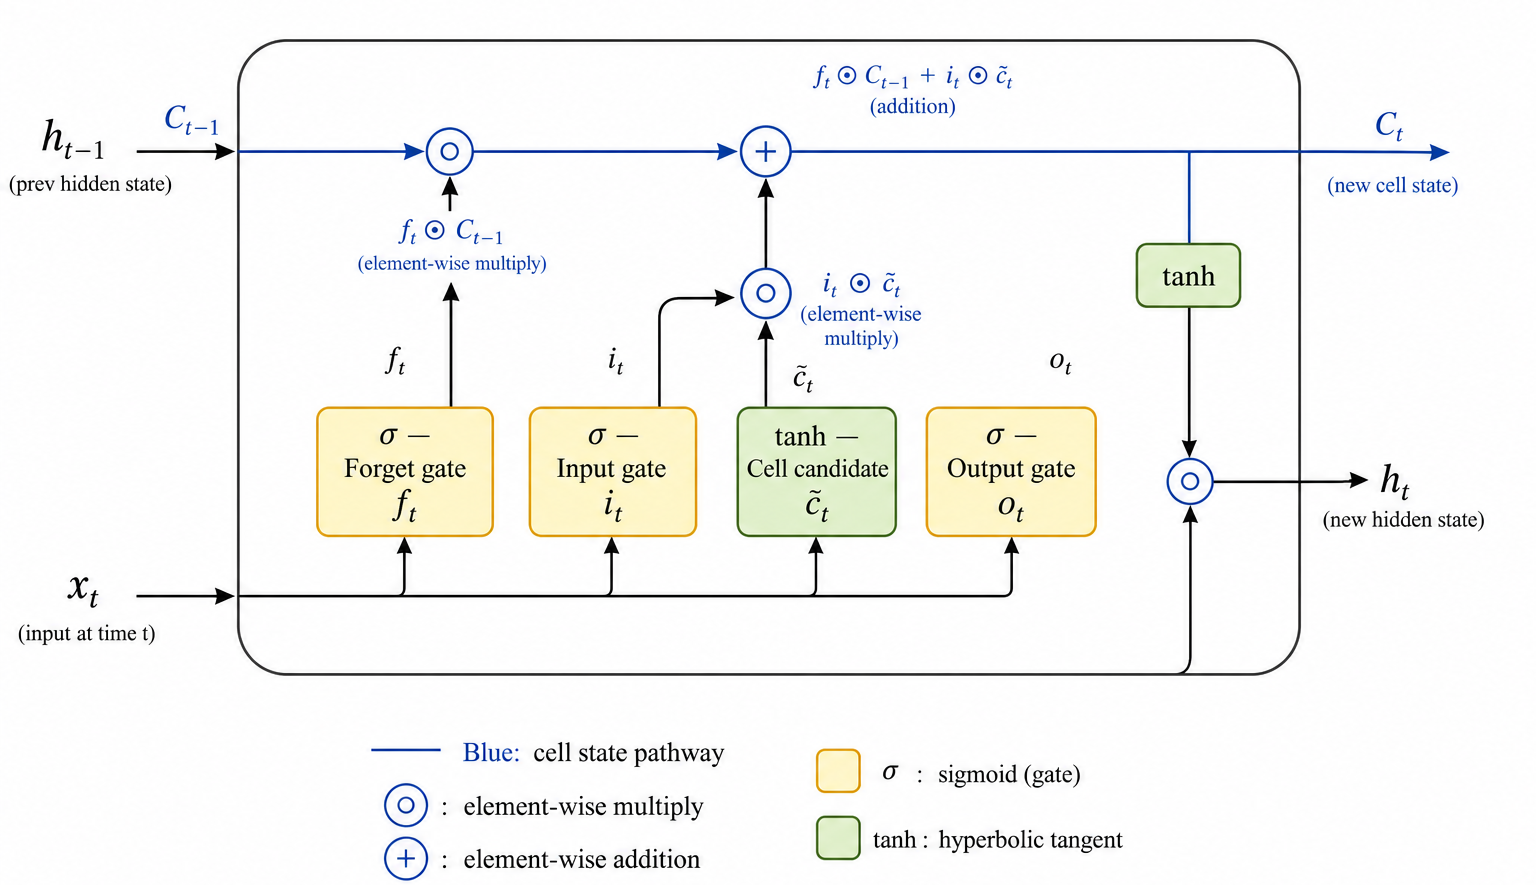
\includegraphics[width=0.99\textwidth]{images/fig_4-11_lstm_cell.png}
\caption{LSTM cell internal structure (Equations~\eqref{eq:ch4-lstm-i}--\eqref{eq:ch4-lstm-h}). The blue cell-state highway $\mathbf{c}_{t-1} \to \mathbf{c}_t$ is gated by the forget gate $\mathbf{f}_t$ (retention) and the input gate $\mathbf{i}_t$ plus candidate $\tilde{\mathbf{c}}_t$ (new content). The output gate $\mathbf{o}_t$ controls how much of $\tanh(\mathbf{c}_t)$ is exposed as the hidden state $\mathbf{h}_t$.}
\label{fig:ch4-lstm-cell}
\end{figure}
\vspace{0.4cm}

\noindent\textbf{4.8.2\quad Bidirectional LSTM:}\par
\addcontentsline{toc}{subsection}{\numberline{4.8.2}Bidirectional LSTM:}
\vspace{0.3cm}

\noindent A BiLSTM runs two independent chains over the sequence --- one forward ($t{=}1\!\to\!T$) and one backward ($t{=}T\!\to\!1$) --- and concatenates both hidden states at every step~\cite{schuster1997bidirectional}:
\begin{equation}
\overrightarrow{\mathbf{h}}_t = \mathrm{LSTM}_{\text{fwd}}(\mathbf{x}_t,\;\overrightarrow{\mathbf{h}}_{t-1}), \qquad \overleftarrow{\mathbf{h}}_t = \mathrm{LSTM}_{\text{bwd}}(\mathbf{x}_t,\;\overleftarrow{\mathbf{h}}_{t+1}),
\label{eq:ch4-bilstm-passes}
\end{equation}
\begin{equation}
\mathbf{h}_t^{\text{bi}} = \bigl[\,\overrightarrow{\mathbf{h}}_t\,;\,\overleftarrow{\mathbf{h}}_t\,\bigr] \in \mathbb{R}^{2h}.
\label{eq:ch4-bilstm-concat}
\end{equation}
Seeing both the sign onset and completion at every time step reduces sensitivity to clip alignment and variable signing speed across signers~\cite{schuster1997bidirectional}.\par\vspace{0.3cm}
\clearpage
\noindent\textbf{4.8.3\quad Full Architecture (Model 4):}\par
\vspace{0.2cm}

\noindent The \texttt{tf.keras.Sequential} model contains exactly four layers:\par\vspace{0.3cm}

\begin{table}[H]
\centering
\caption{ArSL word BiLSTM full architecture (Model~4).}
\label{tab:ch4-bilstm-arch}
\small
\renewcommand{\arraystretch}{1.4} % Adds vertical padding so the text doesn't hit the borders
\begin{tabular}{|c|P{3.8cm}|c|P{2.4cm}|P{4.0cm}|}
\hline
\textbf{Layer \#} & \textbf{Type} & \textbf{Units} & \textbf{Output shape} & \textbf{Notes} \\ \hline
--- & Input & --- & $(48,\;225)$ & $\mathbf{X}' \in \mathbb{R}^{48 \times 225}$ \\ \hline
1 & Bidirectional(LSTM) & 64 & $(48,\;128)$ & \texttt{return\_\allowbreak sequences=True}; concat 64 fwd + 64 bwd \\ \hline
2 & Bidirectional(LSTM) & 64 & $(128)$ & \texttt{return\_\allowbreak sequences=False}; final step only \\ \hline
3 & Dense (ReLU) & 32 & $(32)$ & Affine + ReLU nonlinearity \\ \hline
4 & Dense (Softmax) & 100 & $(100)$ & Class probability distribution \\ \hline
\end{tabular}
\end{table}
\vspace{0.1cm} % Tightened to pull the image up

\begin{figure}[H]
\centering
% Shrunk from 0.72 to 0.65 so it pops back up onto the previous page
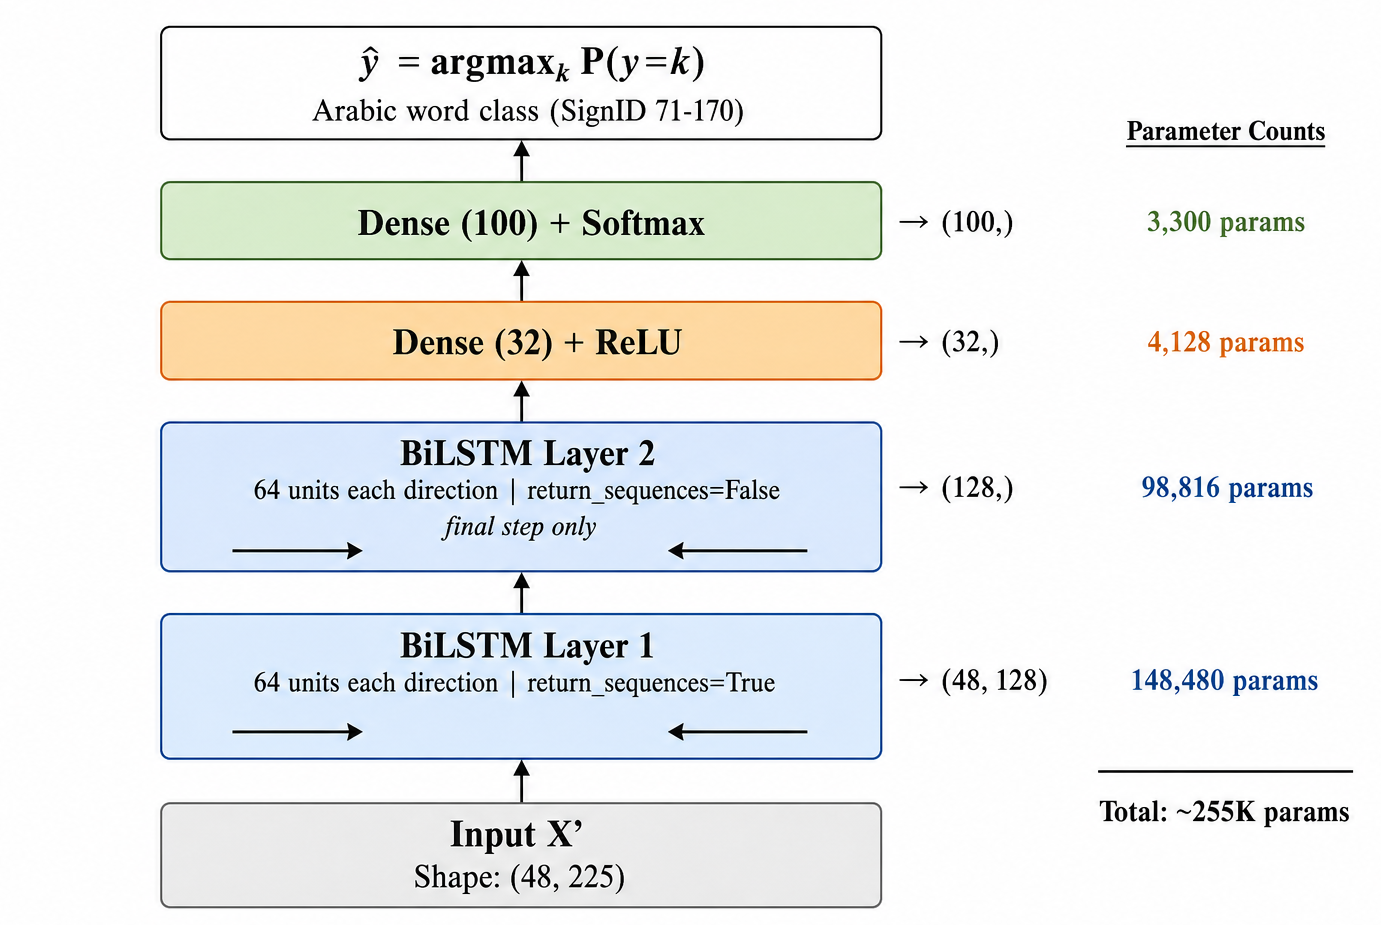
\includegraphics[width=0.71\textwidth]{images/fig_4-12_bilstm_architecture.png}
\caption{ArSL stacked BiLSTM architecture with per-layer output shapes and parameter counts (Table~\ref{tab:ch4-bilstm-arch}). BiLSTM Layer~1 (148\,480 params) returns a per-frame sequence $(48,128)$; Layer~2 (98\,816 params) collapses it to a single 128-D signing summary; Dense(32)+ReLU and Dense(100)+Softmax (7\,428 params total) map to 100 Arabic word class probabilities. Total: $\sim$255\,K parameters.}
\label{fig:ch4-bilstm-arch}
\end{figure}
\vspace{0.4cm}



\noindent\textbf{Forward pass equations.} With input $\mathbf{X}' \in \mathbb{R}^{48 \times 225}$ the four layers compute:
\begin{align}
\mathbf{H}^{(1)} &= \mathrm{BiLSTM}_1\!\bigl(\mathbf{X}',\;h_1{=}64\bigr) \in \mathbb{R}^{48 \times 128}, \label{eq:ch4-L1} \\
\mathbf{h}^{(2)} &= \mathrm{BiLSTM}_2\!\bigl(\mathbf{H}^{(1)},\;h_2{=}64\bigr) \in \mathbb{R}^{128}, \label{eq:ch4-L2} \\
\mathbf{u} &= \mathrm{ReLU}(W_a\,\mathbf{h}^{(2)} + \mathbf{b}_a) \in \mathbb{R}^{32}, \label{eq:ch4-dense1} \\
\mathbf{z} &= W_b\,\mathbf{u} + \mathbf{b}_b \in \mathbb{R}^{100}, \label{eq:ch4-dense2} \\
P(y{=}k \mid \mathbf{X}') &= \frac{\exp(z_k)}{\displaystyle\sum_{j=1}^{100}\exp(z_j)}, \qquad \hat{y} = \arg\max_k P(y{=}k \mid \mathbf{X}'). \label{eq:ch4-bilstm-softmax}
\end{align}

\noindent\textbf{4.8.4\quad Parameter Count:}\par
\addcontentsline{toc}{subsection}{\numberline{4.8.4}Parameter Count:}
\vspace{0.3cm}

\noindent For an LSTM$(h)$ with input $d$, the parameter count per direction is $4(d+h)h + 4h$. Bidirectional doubles this.\par\vspace{0.3cm}

\begin{table}[H]
\centering
\caption{Model~4 parameter breakdown. $d_1{=}225$ (input dim), $h{=}64$ (LSTM units per direction), $d_2{=}128$ (BiLSTM~1 output = $2h$).}
\label{tab:ch4-params}
\small
\begin{tabular}{|P{3.5cm}|P{6.5cm}|r|}
\hline
\textbf{Layer} & \textbf{Formula} & \textbf{Count} \\
\hline
BiLSTM~L1 & $2 \times [4(225+64)\times64 + 4\times64]$ & 148\,480 \\
BiLSTM~L2 & $2 \times [4(128+64)\times64 + 4\times64]$ & 98\,816 \\
Dense(32) & $128\times32 + 32$ & 4\,128 \\
Dense(100) & $32\times100 + 100$ & 3\,300 \\
\hline
\textbf{Total} & & \textbf{254\,724 $\approx$ 255\,K} \\
\hline
\end{tabular}
\end{table}
\vspace{0.4cm}

\noindent The $\sim$255\,K parameter count is two orders of magnitude smaller than the I3D model ($\sim$12.5\,M), reflecting the efficiency of operating on pre-extracted 225-D landmark vectors rather than raw $224\!\times\!224$ RGB frames.\par\vspace{0.3cm}
\clearpage
\noindent\textbf{4.8.5\quad Loss and Training:}\par
\addcontentsline{toc}{subsection}{\numberline{4.8.5}Loss and Training:}
\vspace{0.3cm}

\noindent Training minimises categorical cross-entropy over 100-class one-hot labels:
\begin{equation}
\mathcal{L} = -\sum_{k=1}^{100} y_k \log P(y{=}k \mid \mathbf{X}').
\label{eq:ch4-bilstm-loss}
\end{equation}
Training runs used the software environment in Chapter~3 (Table~\ref{tab:ch3-env}): TensorFlow/Keras on Kaggle GPU for full-sequence extraction and BiLSTM fitting; local 4\,GB CUDA was sufficient for inference prototyping only. The checkpoint filename encodes the converged loss ($\mathcal{L} = 0.026$) and training accuracy (99.625\,\%) at the saved epoch, confirming the model was evaluated on a three-signer held-out partition achieving \textbf{99.62\,\% Top-1 accuracy} on 100 Arabic word classes (SignID 71--170)~\cite{sidig2021karsl}.\par\vspace{0.6cm}

% --- 4.9 ArSL INFERENCE PATH ---
\noindent\textbf{4.9\quad ArSL INFERENCE PATH (End-to-End)}\par
\addcontentsline{toc}{section}{\numberline{4.9}ArSL INFERENCE PATH (END-TO-END)}
\vspace{0.4cm}

\noindent The model-side path from Holistic landmarks to a class probability vector:
\begin{enumerate}
\item MediaPipe Holistic extracts pose and hand landmarks per frame; nose/wrist centreing yields $\mathbf{x}_t \in \mathbb{R}^{225}$ (Equations~\eqref{eq:ch4-adjust-pose}--\eqref{eq:ch4-holvec}).
\item Vectors accumulate in a 48-frame rolling buffer on the client.
\item When the buffer is full and at least one hand is visible, the $(48, 225)$ tensor is forwarded for inference (Chapter~5).
\item The stacked BiLSTM (Equations~\eqref{eq:ch4-L1}--\eqref{eq:ch4-bilstm-softmax}) returns top-$k$ class probabilities.
\end{enumerate}
\vspace{0.3cm}

\noindent Per-request bandwidth is $\approx$43\,KB float32 per 48-frame window ($48 \times 225 \times 4$ bytes), versus several megabytes per second for uncompressed 720p video~\cite{rfc6455}. Deployment artifacts are listed in Table~\ref{tab:ch4-artifacts} (Model~4 row). Results are reported in Chapter~6.\par\vspace{0.6cm}

% ==========================================================
% SHARED SECTIONS
% ==========================================================
\clearpage
% --- 4.10 PIPELINE COMPARISON ---
\noindent\textbf{4.10\quad CROSS-LANGUAGE PIPELINE COMPARISON}\par
\addcontentsline{toc}{section}{\numberline{4.10}CROSS-LANGUAGE PIPELINE COMPARISON}
\vspace{0.4cm}

\noindent The following Table~\ref{tab:ch4-pipeline-compare} contrasts every processing stage of the two word pipelines side by side. Table~\ref{tab:ch4-artifacts} lists the deployment artifacts for both models.\par\vspace{0.2cm}

\begin{table}[H]
\centering
\caption{Detailed cross-language comparison of ASL and ArSL word recognition pipelines.}
\label{tab:ch4-pipeline-compare}
\small
\renewcommand{\arraystretch}{1.2} % Adds vertical padding so the text doesn't hit the borders
\begin{tabular}{|P{3.5cm}|P{5.5cm}|P{5.5cm}|}
\hline
\textbf{Stage} & \textbf{ASL (Model~3 / I3D)} & \textbf{ArSL (Model~4 / BiLSTM)} \\ \hline
Feature source & Raw RGB frames (no MediaPipe) & MediaPipe Holistic (WebAssembly) \\ \hline
Per-frame output & 3$\times$224$\times$224 normalised tensor & 225-D body-relative landmark vector \\ \hline
Normalisation & $(p/255)\times2 - 1 \in [-1,1]$ & Nose-centred pose; wrist-centred hands \\ \hline
Clip / buffer size & 32 frames & 48 frames \\ \hline
Buffer management & \texttt{deque\allowbreak(maxlen=32)}; inference on fill & \texttt{deque\allowbreak(maxlen=48)}; inference if \texttt{has\_hand} \\ \hline
Temporal alignment & Rolling deque (no explicit alignment) & Trim first 48 or repeat-last-frame pad \\ \hline
External scaler & None & None (raw normalised coords) \\ \hline
Model class & Inception I3D (PyTorch) & Stacked BiLSTM (Keras) \\ \hline
Input tensor shape & $(1,3,32,224,224)$ PyTorch & $(1,48,225)$ TensorFlow/Keras \\ \hline
Backbone depth & 19 stages (Table~\ref{tab:ch4-i3d-stack}) & 4 layers (Table~\ref{tab:ch4-bilstm-arch}) \\ \hline
Parameters & $\sim$12.5\,M & $\sim$255\,K \\ \hline
Temporal pooling & Mean of logits over $T_{\text{out}}$ & Final hidden state of BiLSTM~2 \\ \hline
Classification head & 100-class Unit3D ($1\!\times\!1\!\times\!1$) + softmax & Dense(100) + softmax \\ \hline
Stabilisation & Majority vote 6/10, conf$\geq$50\,\%, 1.2\,s & Hand-present gate only \\ \hline
Test Top-1 (100 classes) & \textbf{65.89\,\%} & \textbf{99.62\,\%} \\ \hline
Inference bandwidth & Raw frames encoded (several KB/frame) & $\approx$43\,KB per 48-frame window \\ \hline
\end{tabular}
\end{table}
\vspace{0.4cm}

\begin{table}[H]
\centering
\caption{Deployment artifacts for word recognition (Models~3 and~4).}
\label{tab:ch4-artifacts}
\small
\renewcommand{\arraystretch}{1.8} % Adds vertical padding so the text doesn't hit the borders
\begin{tabular}{|P{2.5cm}|P{5.0cm}|P{6.0cm}|}
\hline
\textbf{Model} & \textbf{Checkpoint / weights} & \textbf{Supporting files} \\ \hline
ASL I3D (M3) & \texttt{asl\_\allowbreak word\_\allowbreak i3d.pt} & 100-class WLASL gloss list \\ \hline
ArSL BiLSTM (M4) & \texttt{arsl\_\allowbreak word\_\allowbreak bilstm.h5} & 100-class Arabic label map (SignID 71--170) \\ \hline
\end{tabular}
\end{table}
\vspace{0.4cm}

\begin{figure}[H]
\centering
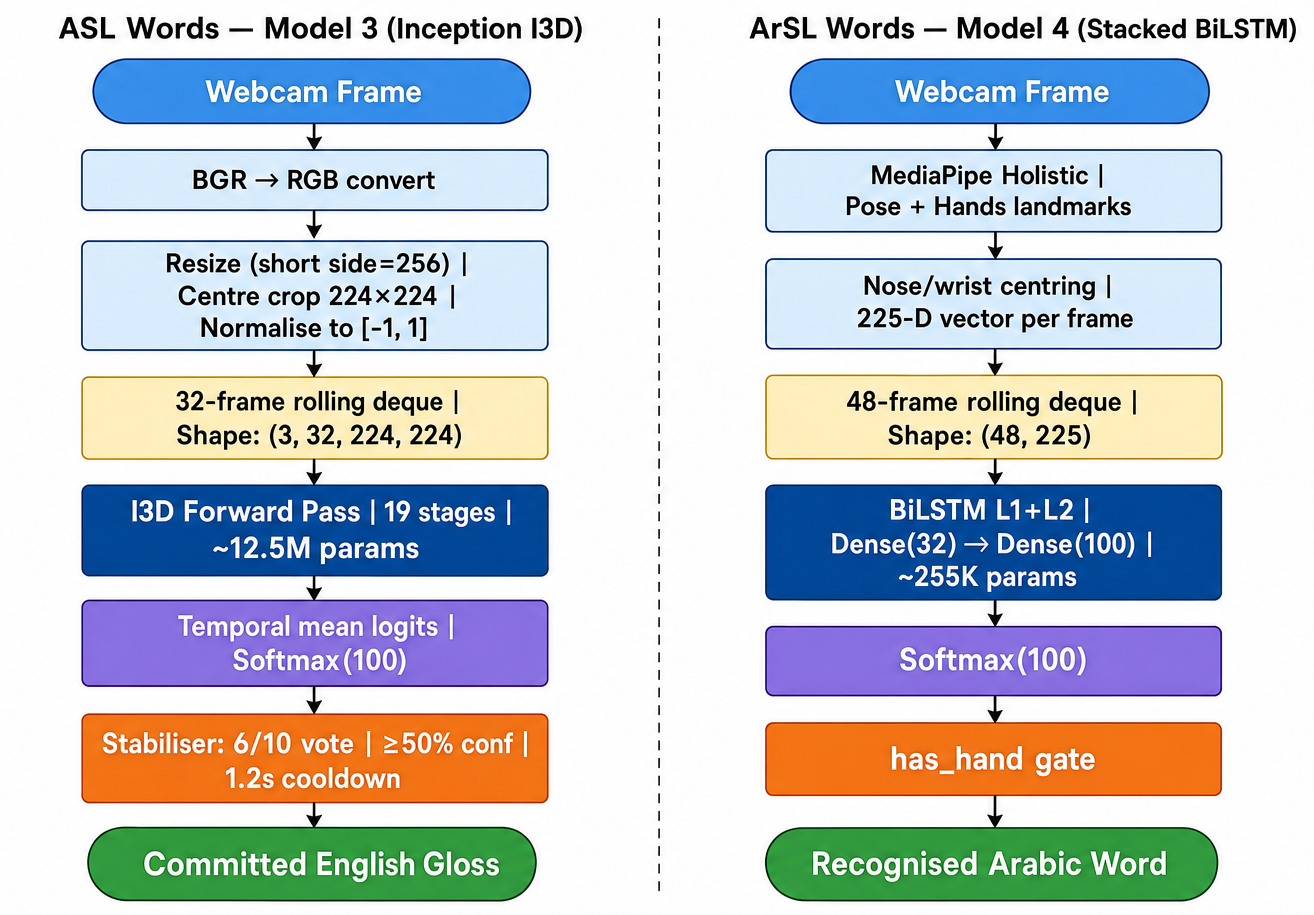
\includegraphics[width=0.99\textwidth]{images/fig_4-13_pipeline_sidebyside.png}
\caption{Side-by-side word inference pipelines for ASL (Model~3, Inception I3D, left) and ArSL (Model~4, Stacked BiLSTM, right). Both pipelines share a rolling-deque temporal buffer and a 100-class softmax output, but differ in feature source (RGB pixels vs.\ Holistic landmarks), buffer depth (32 vs.\ 48 frames), model architecture, parameter count, and stabilisation strategy. See Table~\ref{tab:ch4-pipeline-compare} for a detailed comparison.}
\label{fig:ch4-side-by-side}
\end{figure}
\vspace{0.6cm}
% --- 4.11 TRADE-OFFS ---
\clearpage
\noindent\textbf{4.11\quad ENGINEERING TRADE-OFFS}\par
\addcontentsline{toc}{section}{\numberline{4.11}ENGINEERING TRADE-OFFS}
\vspace{0.4cm}

\noindent Deploying deep neural networks to a live, web-based environment requires carefully balancing theoretical offline accuracy against real-time physical constraints, such as inference latency, memory footprint, and the end user's hardware limitations. Table~\ref{tab:ch4-tradeoffs-asl} records the ASL-specific decisions, where computational cost was traded for the robust spatio-temporal feature extraction of I3D. Conversely, Table~\ref{tab:ch4-tradeoffs-arsl} records the ArSL-specific decisions, which prioritised a lightweight, landmark-based sequence approach suitable for a highly constrained, smaller dataset.\par\vspace{0.4cm}

\begin{table}[H]
\centering
\caption{Engineering trade-offs for ASL word recognition (Model~3).}
\label{tab:ch4-tradeoffs-asl}
\small
\renewcommand{\arraystretch}{1.6} % Adds vertical padding so the text doesn't hit the borders
\begin{tabular}{|P{3.0cm}|P{3.2cm}|P{6.6cm}|}
\hline
\textbf{Decision} & \textbf{Alternative considered} & \textbf{Rationale} \\ \hline
Pretrained I3D (\texttt{asl\_\allowbreak word\_\allowbreak i3d.pt}) & Train BiLSTM+attention from scratch & 4\,GB local GPU; I3D captures spatio-temporal pixel appearance without manual landmark engineering \\ \hline
100-class WLASL subset & Larger offline Holistic experiment & Pretrained I3D is Eshara's deployed ASL word model \\ \hline
Majority vote (6/10) + confidence (50\,\%) & Raw top-1 per clip & Suppresses per-clip noise from mid-gesture frames \\ \hline
1.2\,s cooldown between commits & No cooldown & Prevents the same word triggering twice from a slow signing motion \\ \hline
32-frame deque (not longer) & 64-frame window & Shorter window matches WLASL signing speed and reduces commit latency \\ \hline
\end{tabular}
\end{table}
\vspace{0.4cm}

\begin{table}[H]
\centering
\caption{Engineering trade-offs for ArSL word recognition (Model~4).}
\label{tab:ch4-tradeoffs-arsl}
\small
\renewcommand{\arraystretch}{1.5}
\begin{tabular}{|P{3.0cm}|P{3.2cm}|P{6.6cm}|}
\hline
\textbf{Decision} & \textbf{Alternative considered} & \textbf{Rationale} \\ \hline
Stacked BiLSTM ($\sim$255\,K) & Transformer / full self-attention & $\sim$50 clips/class; BiLSTM generalises reliably with far fewer parameters \\ \hline
225-D nose/wrist-normalised Holistic & Unnormalised pose+hands & Body-relative normalisation reduces camera-distance and signer-height sensitivity \\ \hline
Trim first 48 / repeat-last-frame pad & Uniform temporal resampling & Preserves natural sign endpoints; avoids motion artefacts from frame interpolation \\ \hline
No external scaler & StandardScaler (mean/std per dim) & Model trained on raw normalised coordinates; scaler not saved with checkpoint \\ \hline
48-frame window (vs.\ 32-frame ASL) & Same window for both languages & Average KArSL Arabic word sign is longer than average WLASL English clip~\cite{sidig2021karsl} \\ \hline
100-class KArSL (SignID 71--170) & Full 502-class KArSL & Sample density per class; graduation vocabulary scope \\ \hline
Hand-present gate (\texttt{has\_\allowbreak hand}) & Run inference every frame & Prevents committing on empty frames where no hands are visible \\ \hline
\end{tabular}
\end{table}
\vspace{0.6cm}

% --- 4.12 EVALUATION ---
\noindent\textbf{4.12\quad EVALUATION PROTOCOL (WORDS)}\par
\addcontentsline{toc}{section}{\numberline{4.12}EVALUATION PROTOCOL (WORDS)}
\vspace{0.4cm}

\noindent Each word model is evaluated on a \textbf{held-out test partition} explicitly reserved from the training process or hyperparameter selection phase. Because sign language datasets often suffer from severe class imbalance---where common signs possess significantly more video samples than rare ones---relying solely on Top-1 accuracy can provide a misleading estimate of real-world reliability. Therefore, the evaluation protocol incorporates Top-5 accuracy and Macro-F1 scores to ensure a holistic view of the models' predictive power across all classes, including scarce ones. Table~\ref{tab:ch4-eval-protocol} maps each metric to both models; numeric results appear in Chapter~6~\cite{li2020wlasl,sidig2021karsl,powers2011evaluation}.\par\vspace{0.4cm}

\begin{table}[H]
\centering
\caption{Word-model evaluation protocol (reported in Chapter~6).}
\label{tab:ch4-eval-protocol}
\small
\renewcommand{\arraystretch}{1.6}
\begin{tabular}{|P{3.4cm}|P{5.2cm}|P{5.2cm}|}
\hline
\textbf{Metric} & \textbf{ASL I3D (Model~3)} & \textbf{ArSL BiLSTM (Model~4)} \\ \hline
Top-1 accuracy & WLASL 100-class held-out test & KArSL SignID 71--170 held-out test \\ \hline
Top-5 accuracy & Same test partition & Same test partition \\ \hline
Macro-F1 & Class-balanced summary & Class-balanced summary \\ \hline
Weighted-F1 & Optional secondary metric & Optional secondary metric \\ \hline
Confusion matrix & Per-gloss error analysis & Per-class error analysis \\ \hline
Per-class F1 & Scarce-class diagnosis & Scarce-class diagnosis \\ \hline
End-to-end latency & Live web path (Section~5.12) & Live web path (Section~5.12) \\ \hline
\end{tabular}
\end{table}
\vspace{0.3cm}

\noindent\textbf{ASL word rule:} Top-1 and Top-5 for Model~3 are measured exclusively on the WLASL 100-class held-out test set to ensure no data leakage occurs from the training clips (Chapter~6)~\cite{li2020wlasl}.\par\vspace{0.3cm}

\noindent\textbf{ArSL word rule:} The 99.62\,\% Top-1 metric encoded in the checkpoint filename is derived from the three-signer held-out partition at training time. The full thesis evaluation on KArSL SignID 71--170 test clips rigorously uses the exact preprocessing pipeline established in Sections~4.7.1--4.7.3 (Chapter~6)~\cite{sidig2021karsl}.\par\vspace{0.4cm}

\noindent\textbf{Chapter summary.} \textbf{Part~A (Model~3):} pretrained Inception I3D ($\sim$12.5\,M params) on 32-frame $224\!\times\!224$ RGB clips with majority-vote stabilisation (Tables~\ref{tab:ch4-i3d-stack}, \ref{tab:ch4-stab-params}). \textbf{Part~B (Model~4):} stacked BiLSTM ($\sim$255\,K params) on 48-frame 225-D Holistic sequences for 100 Arabic word classes (Tables~\ref{tab:ch4-bilstm-arch}, \ref{tab:ch4-tradeoffs-arsl}; 99.62\,\% Top-1). Shared deployment artifacts and evaluation protocol are in Tables~\ref{tab:ch4-artifacts} and~\ref{tab:ch4-eval-protocol}. Chapter~6 reports offline accuracy; Chapter~5 reports live web latency.\par

\clearpage